
\subsection{Overview of Numerical Methods}

The availability of powerful computing machines as well as widespread commercial tools allow for coping with engineering problems numerically. Numerical models aim at solving ordinary and partial differential equations with applied initial and boundary conditions by transforming them into a discrete set of algebraic equations. The solution of those algebraic equations leads to an approximate result with respect to the initial PDE's~\cite{eth_introduction_to_finite_element}. The given process is summarised in Fig.~\ref{fig:computational_solution_technique}. 

\begin{figure}[H]
    \renewcommand{\baselinestretch}{0.7} 
    \centering
    \begin{tikzpicture}[node distance = 1.5cm, auto]
        \tikzstyle{decision} = [diamond, draw, fill=blue!20, text width=3cm, text badly centered, node distance=2.5cm, inner sep=0pt, scale=0.8]
        \tikzstyle{block} = [rectangle, draw, fill=blue!20, text width=4.5cm, text centered, rounded corners, node distance=6.0cm, scale=0.8, minimum height=0.5cm]
        \tikzstyle{line} = [draw, -latex']
        \tikzstyle{cloud} = [draw, ellipse,fill=red!20, node distance=3.0cm, minimum height=2em, scale=0.8]
  
    \node [block] (block1) {Proposal of partial differential equations (PDE's) with BC's and IC's};
    \node [block, right of=block1] (block2) {System of algebraic equations};
    \node [block, right of=block2] (block3) {Approximate solution};
    
    \path [line] (block1) -- (block2);
    \path [line] (block2) -- (block3);
    
    \draw [dashed, thin, black, ->] (2.35, 1.5) -- (2.35, 0);
    \draw [dashed, thin, black, ->] (7.1, 1.5) -- (7.1, 0);
    
    \node [draw, ellipse,fill=red!20, minimum height=2em, scale=0.8] at (2.35, 1.5) {Discretisation};
    \node [draw, ellipse,fill=red!20, minimum height=2em, scale=0.8] at (7.1, 1.5) {Equation solver};

    \end{tikzpicture}
    \caption{Schematic of the computational solution technique~\cite{eth_introduction_to_finite_element}.}
    \label{fig:computational_solution_technique}
\end{figure}

Numerical methods have several important advantages. First of all, they allow for finding an approximate solution of a real geometry rather than an exact result of a simplified shape, being the case of analytical analyses. In engineering applications, a numerical analysis serves for parameterising a given technical problem. Therefore, important design factors that influence operating conditions of a developed system may be found and improved. The numerical approach gives answers to so called "what if" questions within a fast iterative thinking process~\cite{heat_transfer_practical_approach_cengel}. There are various numerical methods that serve for conversion of PDE's into a set of algebraic equations such as: 
\begin{itemize}
    \item Finite difference method.
    \item Finite element method.
    \item Finite volume method.
    \item Spectral method.
\end{itemize}

In this thesis, the finite element method (FEM) is employed. It is suitable for solving multi-physical problems as well as the ones characterised by complex geometries, being a case of superconducting magnets. Many commercial numerical tools such as ANSYS or COMSOL use this method because of its capability to solve a large variety of physical problems. 

\subsection{Quench Modelling in Superconducting Magnets}

A quench is a multi-physics problem including among others thermal, electric and magnetic phenomena. In each of these phenomena, one copes with non-linearities of material properties mainly due to a wide range of temperatures at which a magnet operates. From a~design standpoint, a superconducting magnet should sustain a~temperature varying from a~cryogenic one up to the thermal failure limit of an~insulation layer usually remaining in the~limit of a~room temperature. The simulation difficulties covered in this thesis are as follows: 

\begin{enumerate}
    \item Non-linear heat capacity and thermal conductivity of magnet materials. They are a~function of temperature and, in some cases, -- a~magnetic field. 
    \item Non-linear resistivity of copper being a function of temperature and a magnetic field.
    \item Non-linear inductance of a superconducting magnet due to the influence of an iron yoke. 
\end{enumerate}

Apart from a multi-physics environment that requires a coupling of several simulations altogether, the complexity of a quench analysis is also due to the following reasons: 
\begin{enumerate}
    \item Thermal and electrical time constants in transient analyses may vary by several orders of magnitude (multi-rate problem).
    \item Different materials interact with each other, being in some cases also at a varying solid or liquid state if helium is considered (multi-domain problem).
    \item Analysis of components with extremely different sizes may be considered varying from a 10~$\upmu$m-wide filament in a strand to a~10~m-long magnet as a whole (multi-scale problem).
\end{enumerate}

As presented in Fig.~\ref{fig:magnet_design_domains}, the magnet design is an iterative process in which four main studies ought to be conducted: electromagnetic, mechanical as well as the ones related to the quench protection and to the circuit. The change of a design parameter in one element entails the correction of different one in another constituent. As an example, a~study for the quench protection includes the verification whether the magnet does not overheat during the discharge. If the analysis proves a wrong design, the information comes back to electromagnetic studies in which a new design of a coil has to be carried out~\cite{quench_protection_system_applied_prioli}.

\begin{figure}[H]
    \centering
    \begin{tikzpicture}
    \node at (0,0) {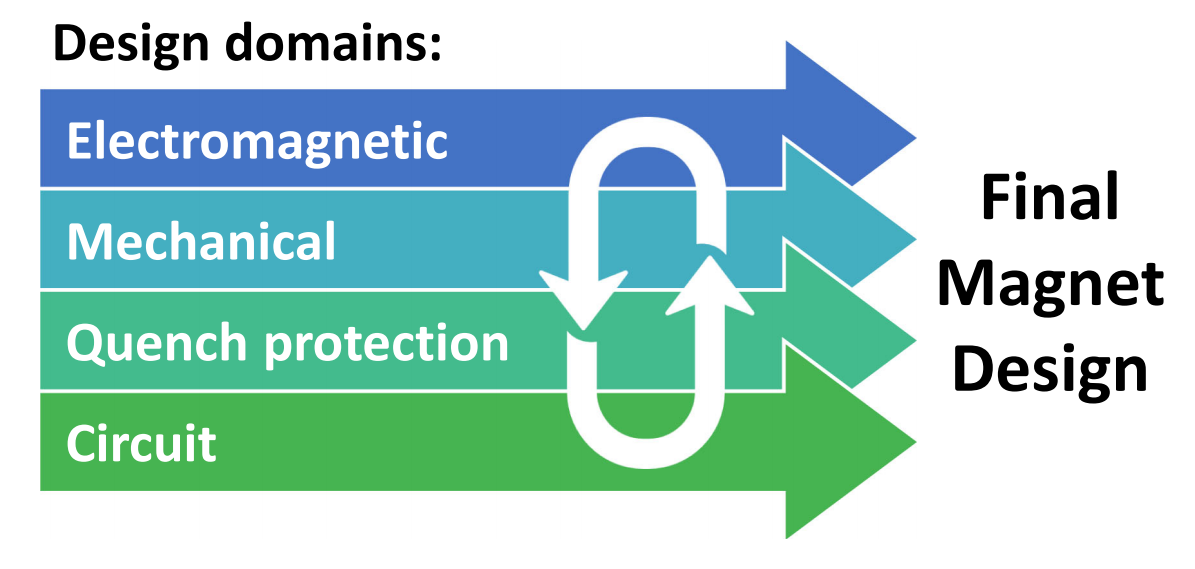
\includegraphics[width=.35\textwidth]{sections/introduction/figures/domains_design_magnet.png}};
    \end{tikzpicture}
    \caption{Domain considered during the design process of a superconducting magnets~\cite{quench_protection_system_applied_prioli}.}
    \label{fig:magnet_design_domains}
\end{figure}

Fig.~\ref{fig:model_complexity_vs_completeness} shows a thermal analysis workflow with respect to the problem complexity from a quench protection perspective. On one hand, the most accurate thermal map of a magnet is desired which allows for lowering the design safety coefficients. However, in order to obtain the most accurate solution, the number of degrees of freedom needs to be increased by applying a denser mesh or an additional dimension in the simulation. The higher completeness of the model is, the longer design iteration loops become. In fact, the iteration loop should be short in order to enable the design process to accelerate . Thus, the modelling approach in a quench protection study is a compromise between the model completeness and the computation time.

\begin{figure}[H]
  \centering
  \begin{tikzpicture}[scale=0.9]
      \begin{polaraxis}
      [
      axis line style = {draw=none}, 
      hide y axis,
      hide x axis,
      no marks,
      samples=201,
      smooth,
      domain=0:2
      ]
      \addplot+ (4*180*x,x);
    \end{polaraxis}
    
    \node[black, scale=0.7] at (3.5,3.2) {0D};
    \node[black, scale=0.7] at (3.5,3.9) {1D};
    \node[black, scale=0.7] at (3.5,2.6) {2D network};
    \node[black, scale=0.7] at (3.5,4.7) {2D FEM};
    \node[black, scale=0.7] at (3.5,1.75) {3D Analytical};
    \node[black, scale=0.7] at (3.3,5.4) {3D FEM + Analytical};
    \node[black, scale=0.7] at (3.35,0.9) {3D FEM};
    \node[black, scale=0.7, text width=2.2cm] at (6.9,3.9) {Model \\ completeness};
    
    \draw[black, ->] (9,1) -- (14,1);
    \draw[black, ->] (9,1) -- (9,4.5);
    \draw[blue] (9,1) .. controls +(10:1cm) and +(-135:1cm) .. (12,2);
    \draw[blue] (12,2) .. controls +(45:1cm) and +(-100:1cm) .. (13,4);
    \node[black, scale=0.7] at (13,0.7) {Model completeness};
    \node[black, scale=0.7, text width=2.3cm] at (10,4.2) {Computation \\ time};
  \end{tikzpicture}
  \caption{Left: thermal analysis workflow with respect to the problem complexity; Right: computation time vs. model complexity~\cite{steam_architecture_presentation}.}
  \label{fig:model_complexity_vs_completeness}
\end{figure}
